\documentclass[11pt, a4paper]{article}
\usepackage[utf8]{inputenc}
\usepackage[spanish]{babel}
\usepackage{graphicx}      
\usepackage{fontspec}
\usepackage{setspace}
\usepackage{anyfontsize}
\usepackage{hyperref}
\hypersetup{
    colorlinks=true,
    linkcolor=black,
    citecolor=magenta,
    urlcolor=cyan,
    pdftitle={Musy Documentación},
    pdfauthor={Beltrán González Martos}
}
\usepackage{listings}
\usepackage{xcolor-material}
\definecolor{codebackground}{rgb}{0.95,0.95,0.95}
\lstset{
    backgroundcolor=\color{codebackground},
    basicstyle=\ttfamily\footnotesize,
    breaklines=true,
    frame=single,
    numbers=left,
    numberstyle=\tiny\color{gray}
}
\onehalfspacing
\setmainfont{IBM Plex Serif}

\begin{document}

\begin{titlepage}
    \centering

    
\includegraphics[width=0.4\textwidth]{media/logo-litterator.png}

    \fontsize{26pt}{24pt}\selectfont \textbf{Trabajo Fin de Grado} \\
    \vspace{4.5cm}
    
    \fontsize{24pt}{24pt}\selectfont \textbf{Musy} \\
    \vspace{0.5cm}
    
\includegraphics[width=0.2\textwidth]{media/Square310x310Logo.png} \\
    \vspace{2cm}

    \hfill
    \begin{minipage}{0.8\textwidth}
        \raggedleft
        \large
        \begin{spacing}{1.5}
            \textbf{Autor:} Beltrán González Martos \\
            \textbf{Tutor:} Héctor Ángeles Borrás \\
            Desarrollo de Aplicaciones Multiplataforma \\
            \textbf{Fecha:} 9 de junio de 2025
        \end{spacing}
    \end{minipage}

    


\end{titlepage}

\pagenumbering{gobble}

\begin{abstract}
    Este proyecto aborda la ausencia de reproductores de musica offline modernos además de abordar el alto consumo de recursos en aplicaciones web, proponiendo una solución basada en tauri (Rust + Angular) para garantizar eficiencia. Se desarrolló una aplicación de escritorio compatible con Linux, MacOs y Windows, priorizando la optimización de memoria y la experiencia de usuario. El resultado es una aplicación escalable con arquitectura modular para futuras extensiones, validando así el potencial de Tauri en aplicaciones de escritorio.
\end{abstract}

\noindent \textbf{Palabras clave}: Tauri, Rust, Angular, reproductor de música, rendimiento, UI moderna, dropdown menu.

\selectlanguage{english}
\begin{abstract}
    This project addresses both the lack of modern offline music players and the high resource consumption in web applications by proposing an efficient solution based on Tauri (Rust + Angular). A cross-platform desktop application was developed for Linux, MacOs, and Windows, with the particular emphasis on memory optimization and user experience. The result is a scalable application with modular architecture for future extensions, demonstrating Tauri's potential for desktop applications.
\end{abstract}

\noindent \textbf{Keywords}: Tauri, Rust, Angular, music player, performance, modern UI, dropdown menu.

\selectlanguage{spanish}

\clearpage

\tableofcontents
\listoffigures
\listoftables
\lstlistoflistings


\clearpage


\pagenumbering{arabic}
\setcounter{page}{1}
\section{Introducción}

Con el aumento de precios y la inclusión de anuncios en las suscripciones premium de plataformas multimedia como Spotify o iTunes, se prevé un resurgimiento de la reproducción local de música. Este proyecto tiene como objetivo ofrecer una alternativa moderna, intuitiva y sencilla frente a las aplicaciones de reproducción local existentes.


\section{Justificación del tema elegido}

Aunque existen alternativas a las aplicaciones de reproducción en streaming, resulta difícil encontrar una que combine una interfaz moderna, atención al detalle y código abierto (open-source). Por ello, se ha desarrollado esta propuesta, centrada en una aplicación de reproducción local con una interfaz similar a Spotify o iTunes, lo que facilitará la transición de nuevos usuarios.

\section{Objetivos}

El objetivo principal es desarrollar una aplicación multiplataforma basada en tecnologías web, eficiente en la gestión de recursos del sistema y fácil de usar. Adicionalmente, se busca que el proyecto sirva como aprendizaje en el uso de Angular y Rust.

\section{Metodología}

Para la realización del proyecto se empleará la metodología ágil SCRUM. En este caso, el autor asumirá los roles de product owner, scrum master y development team. Las tareas serán asignadas diariamente, y se realizará un seguimiento continuo del progreso.

\section{Tecnologías y herramientas usadas en el proyecto}

Este proyecto está desarrollado mediante un conjunto de tecnologías modernas
distribuidas en tres capas principales:

    \begin{itemize}
        \item \textbf{Frontend}: Angular 17, Tailwind CSS V4
        \item \textbf{Backend}: Rust, Tauri 2.0
        \item \textbf{Base de Datos}: SQLite
    \end{itemize}

    \subsection{Razones}

    La selección de tecnologías para este proyecto se ha basado en los siguientes criterios técnicos y de eficiencia: 

        \begin{itemize}
            \item \textbf{Angular 17}: Se ha elegido este framework por su arquitectura basada en componentes, que favorece la escalabilidad y mantenibilidad del código. Además, se ha considerado relevante la oportunidad de explorar alternativas a React, ampliando así el conocimiento en ecosistemas frontend modernos.
            \item \textbf{Tailwind CSS v4}: Se ha optado por esta herramienta debido a su eficiencia en el desarrollo de interfaces responsive, así como a la familiaridad previa con su paradigma utility-first, lo que permite agilizar el proceso de diseño.
            \item \textbf{Rust}: Se ha seleccionado este lenguaje por su rendimiento optimizado y seguridad. Además, representa una valiosa oportunidad de aprendizaje de un lenguaje de programación de bajo nivel.
            \item \textbf{Tauri}: Se ha preferido sobre alternativas como Electron debido a su menor consumo de recursos y mejor rendimiento en aplicaciones de escritorio multiplataforma.
            \item \textbf{SQLite}: Se ha implementado este sistema de gestión de bases de datos por su ligereza, y adecuación a los requisitos del proyecto.
        \end{itemize}

    El entorno de desarrollo está configurado en Visual Studio Code, utilizando extensiones específicas para cada tecnología mencionada, lo que garantiza un flujo de trabajo eficiente.

\section{Especificación de Requisitos de Software}



\section{Despliegue y pruebas}

En este apartado se detallan los pasos seguidos para el despliegue de la aplicación de escritorio, así como las pruebas realizadas para garantizar su correcto funcionamiento.

        \subsection{Despliegue de la aplicación}

        Se elaboró un proceso de empaquetado y distribución de la aplicación utilizando Tauri, que permite generar ejecutables multiplataforma (Windows, MacOs, Linux). Para ello:

        \begin{itemize}
            \item Se utilizó el sistema de bundling de Tauri para empaquetar los recursos frontend (Angular) junto al backend (Rust).
            \item Se generaron instaladores específicos para diferentes sistemas operativos: \begin{itemize}
                \item \textbf{.AppImage} para Linux
                \item \textbf{.exe} para Windows
                \item \textbf{.dmg} para MacOs
                \end{itemize}
        \end{itemize}

        \subsection{Pruebas realizadas}

        Con el objetivo de validar la funcionalidad y estabilidad de la aplicación, se llevaron a cabo las siguientes pruebas:

            \subsubsection{Pruebas de integración}

            \begin{itemize}
                \item Se comprobó la comunicación entre el frontend y el backend, asegurando que las llamadas desde Angular a Rust (a través de Tauri) funcionaban correctamente.
                \item Se testearon casos como la carga de archivos de audio, reproducción en diferentes formatos y manejo de errores.
            \end{itemize}

            \subsubsection{Pruebas de usabilidad}

            \begin{itemize}
                \item Se realizaron test con usuarios reales para evaluar la experiencia de uso (UX), recogiendo feedback sobre la interfaz y la fluidez de la reproducción musical.
                \item Se analizaron posibles cuellos de botella en el rendimiento, especialmente al manejar playlist con muchas canciones o archivos de alta resolución.
            \end{itemize}

        La aplicación fue testeada en los tres sistemas operativos principales (Windows, MacOs y Linux), aunque el desarrollo se centró principalmente en las versiones para MacOs y Linux. \\

        El rendimiento de la aplicación resulta significativamente mejorado al aprovechar las características nativas de Tauri, en comparación con soluciones basadas en Electron. \\

        \begin{figure}[h!]
            \centering
            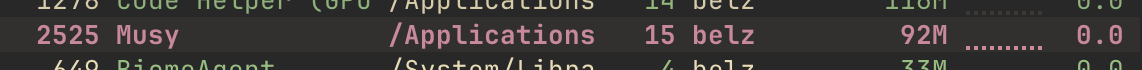
\includegraphics[width=0.8\textwidth]{media/imagemusyram.png}
            \caption{Rendimiento de la aplicación en MacOs}
            \label{fig:ejemplo}
        \end{figure}

\section{Estado del arte}

En la actualidad, el panorama de reproducción musical se divide principalmente en dos enfoques: plataformas de streaming y reproductores locales tradicionales. A continuación, se analizan sus características, ventajas y desventajas.

        \subsection{Plataformas de streaming}

        Las plataformas de streaming (Spotify, Apple Music, etc...) dominan el mercado actual debido a:

        \begin{itemize}
            \item Acceso instantáneo a catálogos musicales extensos (más de 100 millones de canciones).
            \item Interfaces modernas con recomendaciones basadas en algoritmos.
            \item Sincronización multiplataforma (dispositivos móviles, web y escritorio).
        \end{itemize}

        Sin embargo, presentan limitaciones significativas:

        \begin{itemize}
            \item Dependencia de conexión a internet permanente.
            \item Modelo de negiocio basado en suscripciones o publicidad invasiva.
            \item Falta de propiedad real sobre la música (acceso condicionado al pago).
        \end{itemize}

        \subsection{Reproductores locales tradicionales}

        Los reproductores de música offline (Winamp, Strawberry, etc...) ofrecen:

        \begin{itemize}
            \item Control completo sobre los archivos musicales (propiedad permanente).
            \item Uso sin restricciones de conectividad o cuentas de usuario.
            \item Menor consumo de recursos al evitar dependencias en la nube.
        \end{itemize}

        No obstante, adolecen de problemas críticos:

        \begin{itemize}
            \item Interfaces obsoletas y experiencias de usuario poco intuitivas.
            \item Dificultad para encontrar versiones actualizadas (muchos proyectos estan abandonados).
            \item Limitada compatibilidad con formatos modernos o sistemas operativos recientes.
        \end{itemize}

        \subsection{Mi propuesta}

        Este análisis evidencia la necesidad de reproductores locales que combinen:

        \begin{itemize}
            \item Diseño contemporáneo (similar al streaming).
            \item Independencia de infraestructuras en la nube.
            \item Soporten estándares actuales (formatos lossless, metadatos avanzados).
        \end{itemize}

        La solución propuesta en este proyecto busca ocupar este espacio, aprovechando tecnologías modernas (Tauri, Rust, Angular) para superar las limitaciones de ambas aproximaciones.

\section{Profundización de conceptos}

En esta sección se explicarán en detalle los componentes principales de la aplicación.

        \subsection{Frontend}

        Angular

            \subsubsection{Playbar}

            Componente principal para la reproducción de música, esta compuesto por 3 divs:

            \begin{itemize}
                \item \textbf{Izquierdo}. Aquí se encuentran la foto de la canción, el título y el artista.
                \item \textbf{Central}. Contiene otros 2 divs mas pequeños, uno para los botones de play, pause, shuffle, last song, next song, repeat; y otro para la barra de reproducción. Más adelante se explicarán cada uno de ellos en el apartado de servicios.
                \item \textbf{Derecho}.Este div unicamente contiene la barra para ajustar el volumen. A futuro es posible que se implemente un botón para abrir el menú de la cola e interactuar con ella.
            \end{itemize}

            La parte del componente de typescript contiene únicamente métododos que llaman al servicio de manejo de canciones \verb|song-management.service.ts|.

            \subsubsection{Sidebar}

            Componente donde se interactua con las playlist, ya sea creando nuevas o borrando las existentes. Contiene diversos botones para navegar por la aplicación.

                \paragraph{Playlist}
                ‎ 

                \begin{lstlisting}[caption={Atributos y Constructora}]
coverPath = 'assets/black.jpg';

isDropDownOpen: boolean = false;

constructor (public mainScreenStatus:MainScreenStatusService) {}

@Input() playlistId!: number;

@Input() playlistName!: string;

@Input() playlistDate!: string;

@Input() playlistCoverPath!: string;

@Input() playlistIsStarred!: boolean;

@Input() refreshFn!: () => void;
                \end{lstlisting}

                Cada playlist es un botón que cambia el contenido de la \verb|mainscreen|, enviando la lista de canciones a ese componente mediante un servicio. Algunos de los métodos más importantes de este componente son:

                \begin{lstlisting}[caption={getCoverPath()}]

async getCoverPath(): Promise<string> {
    if (!this.coverPath) return 'assets/black.jpg';
    console.log("Hola")

    const fileData = await readFile(this.playlistCoverPath);
        
    const blob = new Blob([fileData], { type: 'image/jpeg' });

    if (this.coverPath) {
        URL.revokeObjectURL(this.coverPath);
    }

    return URL.createObjectURL(blob);
}
                \end{lstlisting}

                Debido a que la ruta de la portada no es válida para ser mostrada directamente, hay que convertirla en un blob. Este método se encarga de ello, y, en el caso de que no exista una portada retorna una imagen default.

                \begin{lstlisting}[caption={Dropdown}]
toggleDropDown() {
    this.isDropDownOpen = !this.isDropDownOpen;
  }

  closeDropDown() {
    this.isDropDownOpen = false;
  }

  @HostListener('document:click', ['$event'])
  onClickOutside(event: Event) {
    const target = event.target as HTMLElement;
    if (!target.closest('.relative.inline-block')) {
      this.closeDropDown();
    }
  }
                \end{lstlisting}

                Por temas de diseño, se ha decidido crear un dropdown menu donde aparecerá el boton de eliminar playlist. A futuro es posible que se implementen más botones como por ejemplo para añadir una playlist a favoritos.

                \begin{lstlisting}[caption={removePlaylist()}]
async removePlaylist() {
    const data_dir = await appDataDir();
    invoke('remove_playlist', {playlist_id: this.playlistId, db_path: data_dir});
    this.refreshFn();
  }
                \end{lstlisting}

                Para eliminar una playlist de la sidebar se hace una llamada al backend donde se realizará una consulta sql para eliminarla de la base de datos (Esto se verá mas adelante en el apartado de Rust y SQL).

            \subsubsection{Mainscreen}

            \subsubsection{Servicios}

        \subsection{Backend}

        Rust y SQLite

            \subsubsection{Tauri API}

            \subsubsection{Sync method}

            \subsubsection{SQL CRUD}


\section{Conclusiones}

        \subsection{Logros principales}

        Se ha desarrollado con éxito un reproductor de música multiplataforma (Linux, MacOs y Windows) utilizando Tauri, que cumple con los objetivos principales de:

        \begin{itemize}
            \item Optimización de recursos (Mucho menor consumo de ram respecto a otras webapps basadas en Electro).
            \item Compatibilidad de formatos de audio (FLAC, MP3, etc...).
            \item Arquitectura modular para el desarrollo futuro.
        \end{itemize}

        \subsection{Dificultades clave}

        El principal desafío técnico fue la curva de aprendizaje asociada a Rust, lenguaje de programación de sistemas con el que no se contaba experiencia previa. Esta dificultad se resolvió mediante el estudio de documentación oficial, tutoriales especializados y la implementación de pruebas piloto. Adicionalmente, fue necesario adaptar los conocimientos existentes en desarrollo web al framework Angular, cuyo paradigma de componentes requirió un período de adaptación.

        \subsection{Valoración global}

        A pesar de las dificultades, el proyecto valida el potencial de Tauri para aplicaciones de audio eficientes, ofreciendo un rendimiento superior al de frameworks tradicionales. La escalabilidad de la arquitectura permite añadir funcionalidades como cambios en la apariencia en futuras iteraciones.

\end{document}